% !TeX root = ../main.tex

\chapter{Real time reccurent learning}

A partir de cette section, les objectifs sont de reconnaître une chaine de caractère en temps réel : c'est à dire que en donnant un ou plusieurs caractères , on doit être capable de prédire la fin de la chaine.
Ce genre de problème peut être étendu à la recherche comportementale en temps réel.
Pour résoudre ce genre de problème, on utilise des réseaux neuronaux récurrents, qui ont l'avantage de se souvenir des états précédents pour pouvoir prédire efficacement les états suivants; ils comportent une mémoire courte.
Dans un premier temps, nous allons nous intéresser aux réseaux RTRL.

\section{Théorie}

Dans la suite, nous allons nous intéresser au problème de la grammaire de Reber, qui servira d'échantillon de test pour RTRL.

\subsection{La grammaire de Reber}

Une grammaire de Reber est un langage défini par l'automate déterministe cyclique suivant :

\begin{figure}[!ht]
\begin{center}
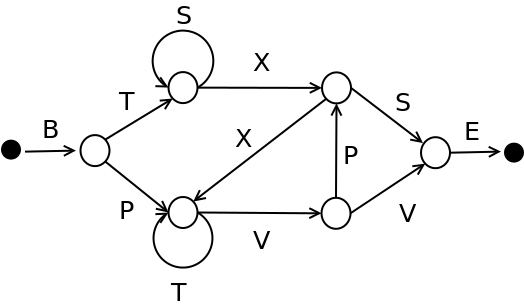
\includegraphics[scale=0.4]{images/reberGrammar.png}
\end{center}
\caption{Grammaire de Reber simple}
\end{figure}


De base, on considère une probabilité uniforme de choisir l'état suivant parmi les états possibles suivants.
La lettre $B$ et la lettre $E$ sont des lettres indiquant simplement le début et la fin de la chaîne, elles n'ont pas d'intérêt propre pour la grammaire.
Les autres lettres présentes sur les arêtes peuvent variées, mais elles doivent respecter les règles suivantes :
\medskip
\begin{itemize}
	\item Chaque lettre doit apparaitre exactement deux fois
	\item On ne peut pas obtenir deux lettres consécutives en passant par des états différents.
\end{itemize}
\vspace{\parskip}
L'intérêt de la grammaire de Reber est que c'est un automate simple qui ne nécessite que la mémoire de la dernière et de l'avant dernière lettre pour trouver la suivante.
En effet, d'après la dernière règle, connaitre les deux dernières lettres impose l'état actuel dans l'automate.
En outre, chaque lettre apparaissant deux fois, la connaissance seule de la dernière lettre ne suffit pas à prédire la suivante correctement.
On remarque que l'on peut résoudre ce problème avec un perceptron classique si on donne en entrée du perceptron les deux dernières lettres du mot.
Ce modèle bien que résolvant ce problème, n'est pas adapté au calcul en temps réel.
De plus il ne résout pas le problème de la grammaire de Reber double.

Le problème de la grammaire double est un problème similaire à la grammaire
simple. L'automate le représentant est :

\begin{figure}[!ht]
\begin{center}
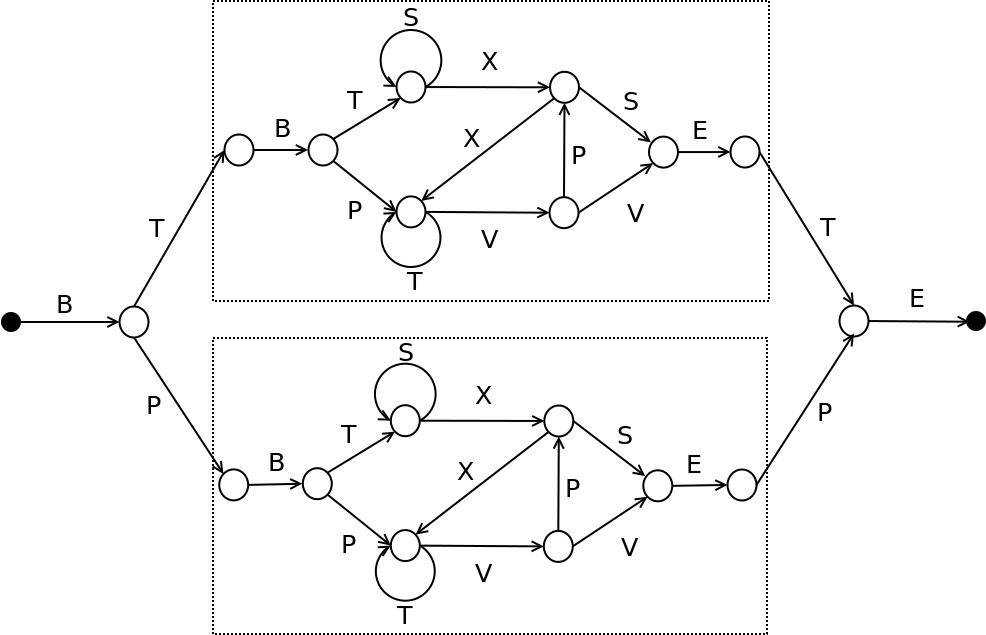
\includegraphics[scale=0.4]{images/reberGrammarSymmetric.png}
\end{center}
\caption{Grammaire de Reber symétrique}
\end{figure}

On remarque qu'il est constitué de deux grammaires de Reber simple qui sont reliés en entrée et en sortie.
La difficulté de ce problème est qu'il faut mémorisé la première valeur pour en déduire la dernière.
Dans ce cas, une mémoire ''infini'' est nécessaire théoriquement pour se souvenir de la première entrée.
Il est donc impensable d'utiliser de la même façon un réseau de perceptron classique. On a alors besoin de réseau récurrent, dont la sortie à un instant $t$ va dépendre de la sortie à un instant $t-1$.

\subsection{Réseau RTRL}

Le principe d'un réseau récurrent est d'utiliser le résultat obtenue par la sortie précédente à l'entrée du calcul suivant.
On aura donc en appelant $x(t)$ la donnée en entrée à l'instant $t$ et $y(t)$ la sortie associé.
On a alors $y(t) = f(x(t), y(t-1))$.
En appelant $\alpha$ un paramètre de la fonction $f$.
Le but est de faire un apprentissage sur $\alpha$ pour minimiser à chaque temps $t$ l'erreur $E(t)$ entre la sortie théorique et la sortie pratique.
De la même façon que précédemment, on va donc calculer $\cfrac{\partial E(t)}{\partial \alpha}$ pour utiliser la méthode du gradient :
Dans un premier temps, nous allons nous intéresser au cas où $f$ est de la forme :

\[ f(x(t), y(t-1)) = \sigma\left (W x(t) + R y(t-1) + b\right )\]

Avec $W$, $R$ qui sont des matrices de poids, $b$ un biais et $\sigma$ une fonction d'activation.
On reconnait donc d'après ce qui précède la formule d'un réseau perceptron à $0$ couche caché et "fully connected".
On pose $\overline{y(t)} = W\times x(t) + R\times y(t-1) + b$.
Les paramètres du systèmes sont donc les éléments de la matrice
On obtient donc pour l'apprentissage :

\[\cfrac{\partial E(t)}{\partial \alpha} = \left\langle \cfrac{\partial y(t)}{\partial \alpha}, J_E \right\rangle\]

\begin{figure}[!ht]
\begin{center}
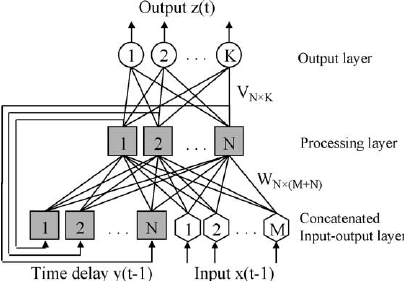
\includegraphics[scale=0.8]{images/rtrl.png}
\end{center}
\caption{Réseau récurrent RTRL}
\end{figure}

\section{Implémentation}

\section{Résultats}
\subsection{Grammaire de Reber simple}
\subsection{Grammaire de Reber double}
